 %In order to solve our new task, we would expect our classifier to get improved performance with respect to
%\begin{itemize}
%\item Exploiting knowledge from related source models. If these two tasks are related, SMITLe should transfer the prior knowledge aggressively. In some cases where the prior knowledge is very related and training size of the target task is small, the final decision of the classifier could be mainly rely on the decision from the source models.
%\item Disposing unrelated knowledge. If the knowledge between these two tasks is unrelated, the algorithm should be able to distinguish and dispose the unrelated knowledge autonomously. In the worst case, none of the prior knowledge is related and SMITLe should show similar performance as the model trained merely from target data.
%\end{itemize}

%In this paper, we use LS-SVM as the classifier for the multi-class incremental transfer problem. In the following, we briefly introduce the mathematical setting of our problem.

In this section, we focus on the Phrase I of HTL and introduce our biased regularization for binary LS-SVM for our problem. We use multi-source transfer strategy to generate our biased regularization. As a result, the decision of each binary LS-SVM is the linear combination of the knowledge from both target task and source hypotheses controlled by certain transfer parameters.

We define our task in the following way: assume that, for our $(N+1)$-category target task, ${x} \in \mathcal{X}$ and ${y} \in Y=\left\{1,2,...,N+1\right\}$ are the input vector and output for the learning task respectively. Meanwhile, we have a set of binary linear classifiers (hypotheses) $f'_n(x)=\phi(x)w_n'+b_n'$, for $n=1,...,N$ trained from an unknown distribution with One-Versus-All (OVA) strategy.  Now we want to learn a set of classifiers $f_n(x)=\phi(x)w_n+b_n, n=1,...,N+1$ for our new task. The example $x$ is assigned to the category $j$ if $j \equiv \arg {\max _{n = 1,...,N+1}}\left\{{f_n}(x)\right\}$. From previous works of HTL, the solution of the parameters $(w_n,b_n)$, for each binary LS-SVM, can be found by solving the following optimization problem:
\begin{equation*}
\begin{aligned}
\textbf{min} && R({w_n,W'}) + \frac{C}{2}\sum\limits_i^l {({Y_{i,n}} - \phi ({x_i}){w_n} - {b_n})^2} \\
\end{aligned}
\end{equation*}
Here, $W'=\{w_1',w_2',...,w_n'\}$. $R({w_n,W'})$ is the regularization term to guarantee good transfer performance and avoid overfitting. $\mathbf{Y}$ is a encoded label matrix so that $Y_{in}=1$ if $y_i=n$ and $-1$ otherwise.


Now our task can be divided into two separate part: learning the the $(N+1)_{th}$ new category and $N$ overlapped categories.

For the new added category, it is very difficult to identify the utility of the hypothesis of a single category in source task, therefore, we use multi-source transfer strategy, adopted from Multi-KT \cite{tommasi2014learning}, to leverage hypotheses from multiple sources. As a result, regularization term $R(w_{N+1},W')$ can be written as:
\begin{equation}
\begin{aligned}
R(w_{N+1},W')= \frac{1}{2}{\left\| {{w_{N + 1}} - \sum\limits_{k = 1}^N {w{'_k}{\beta _k}} } \right\|^2} 
\end{aligned}\label{eq:multi}
\end{equation}
We can interpret the biased regularization in the following way. Let $w_{N+1} = w_{N+1}''+\sum\limits{\beta _kw'_k}$ (See Figure \ref{fig:combine}). Therefore, we have:
\begin{equation*}
w_{N+1}\phi(x)=w_{N+1}''\phi(x)+\sum\limits{\beta _kw'_k\phi(x)}
\end{equation*}

\begin{figure}
\centering
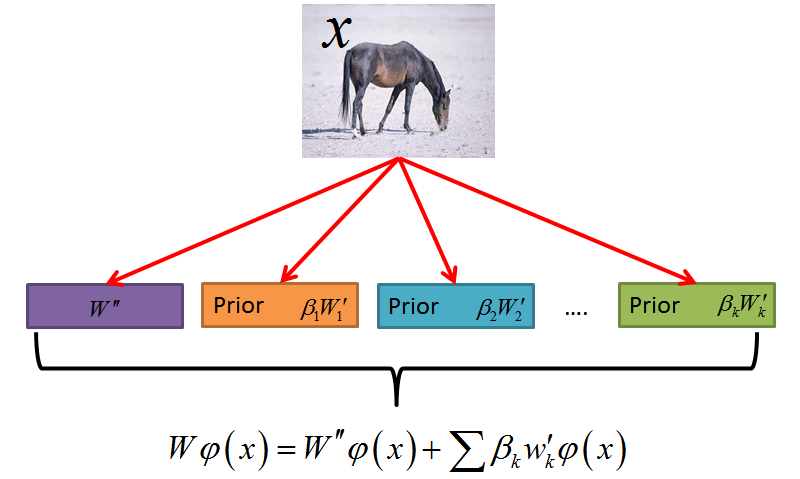
\includegraphics[scale=0.25]{fig/combine.png}
\caption{The final decision function value of a binary SVM can be get by combining the prior and empirical knowledge.}\label{fig:combine}
\end{figure}
Here, we call $\beta$ the transfer parameter. For any fixed value of $\beta$, regularizing $w_n$ is equivalent to regularize $w_{N+1}''$, i.e. $(w_{N+1}-\sum\limits{\beta _kw'_k})$. The decision of each binary SVM model is made by combining the decision from target task $w_{N+1}''\phi(x)$ and source hypotheses $w'_k\phi(x)$ controlled by the transfer parameter. The amount of transfered knowledge has a positive correlation to the value of $\beta$.

However, for the original $N$ categories, we already have their corresponding source category hypotheses and thus, their regularization term can be written as:
\begin{equation}\label{eq:asvm}
\begin{aligned}
R(w_n,w_n')= \frac{1}{2}{{{\left\| {{w_n} - {\gamma _n}{{w'}_n}} \right\|}^2}}  
\end{aligned}
\end{equation}
As we can see that the regularization term \eqref{eq:asvm} is a special case of \eqref{eq:multi} where only one $\beta_k$ is none-zero. 

Combining these two together, our multi-class incremental transfer problem can be solved by optimizing the following objective function:
\begin{equation}
\begin{aligned}
\textbf{min}\qquad {} & \frac{1}{2}\sum\limits_{n = 1}^N {{{\left\| {{w_n} - {\gamma _n}{{w'}_n}} \right\|}^2}}  + \frac{1}{2}{\left\| {{w_{N + 1}} - \sum\limits_{k = 1}^N {w{'_k}{\beta _k}} } \right\|^2}\\& +\frac{C}{2}\sum\limits_{n = 1}^{N + 1} {\sum\limits_{i = 1}^l {e_{i,n}^2} }  \\
\textbf{s.t.}\qquad {} &{e_{i,n}} = {Y_{in}} - \phi ({x_i}){w_n} - {b_n}, \quad n \in \{1,...,N+1\}
\end{aligned}\label{eq:opt}
\end{equation}

The optimal solution to  Eq. (\ref{eq:opt}) is:
\begin{equation}\label{eq:solu}
\begin{aligned}
{w_n}&= {\gamma _n}{{w'}_n} + \sum\limits_i^l {{\alpha _{in}}{\phi(x_i)}} ,{n = 1,...,N}\\
{w_{N + 1}}&= \sum\limits_k^N {{\beta _k}{{w'}_k}}  + \sum\limits_i^l {{\alpha _{i(N + 1)}}{\phi(x_i)}} 
\end{aligned}
\end{equation}
Here $\alpha_{ij}$ is the element $(i,j)$ in $\boldsymbol{\alpha}$. 

Let $K(X,X)$ be the kernel matrix and
\begin{equation}\label{eq:linear}
\psi=\left[ {\begin{array}{*{20}{c}}
{K(X,X) + \frac{1}{C}{\rm{I}}}&\mathbf{1}\\
\mathbf{1^T}&0
\end{array}} \right]
\end{equation}

\begin{equation}
\begin{array}{c}
 {\psi}\left[ {\begin{array}{*{20}{c}}
{\boldsymbol{\alpha} '}\\
{\boldsymbol{b}'}
\end{array}} \right] = \left[ {\begin{array}{*{20}{c}}
Y\\
0
\end{array}} \right], \quad
{\psi}\left[ {\begin{array}{*{20}{c}}
{\boldsymbol{\alpha} ''}\\
{\boldsymbol{b}''}
\end{array}} \right] = \left[ {\begin{array}{*{20}{c}}
{X{{\left( {W'} \right)}^T}}\\
0
\end{array}} \right]
\end{array}
\end{equation}
We have:
\begin{equation}\label{eq:solution}
 \boldsymbol{\alpha}  = \boldsymbol{\alpha} ' - \left[ {\begin{array}{*{20}{c}}
 {\boldsymbol{\alpha} ''\boldsymbol{d_{\gamma}}}&{{\boldsymbol{\alpha} ''\boldsymbol{\beta ^T}}}
 \end{array}} \right]
\end{equation}
Here $\boldsymbol{d_{\gamma}}$ is a diagonal matrix with $\{\gamma_i\}_{i=1,...,N}$ in its main diagonal. From Eq. (\ref{eq:solution}) we can see that, the solution of Eq. (\ref{eq:opt}) is completed once $\boldsymbol{\gamma}$ and $\boldsymbol{\beta}$ are set.

